\section{Myoblast Segmentation using \stardist}\label{secstardist}
As discussed in Sec.~\ref{secunsupervised}, typical instance segmentation methods suffer from the suppresion of valid objects or the merging of instances given overlaps. In order to better segment the myoblasts, a cell detection method called \stardist \cite{schmidt2018, weigert2020} is used. It was developed with the intent to segment microscopy data like the nuclei found in this project. A deep learning model would have the advantage of being flexible enough to not require much preprocessing and can ideally be used out-of-box if there exists a pretrained model.
\subsection{\texttt{StarDist} Background}
In brief, a convolutional neural network is trained to predict polygons imitating typical cell shapes for every pixel of the image. More concretely, it predicts a star-convex polygon for every (non-background) pixel. Intuitively speaking, a star-convex set $\mathcal{S}$ is one where there exists one point $s_{0}$ such that for every point $s \in \mathcal{S}$ the line segment connecting $s_{0}$ to $s$ is element of $\mathcal{S}$. Such a shape can be approximated by following $n$ predefined radial directions for a distance of $\{r^{k}\}^{n}_{k = 1}$ starting from a point $s_{0}$. This better approximates the myoblast shape than ellipses. The training data contains pairs of both raw and fully annoted label images in the sense that every pixel either has a unique object identifier or is marked as background. Given the annoted images, it is possible to compute the radial distances $\{r^{k}_{ij}\}^{n}_{k = 1}$ to the assigned object's boundaries starting at every single foreground pixel parametrized by $i, j$ serving as the point  $s_{0}$. Furthermore, for every single foreground pixel the Euclidean distance to the closest background pixel is computed. Normalizing this distance gives a value $d_{ij}$ between 0 and 1 interpreted as a probability to be a foreground point. The calculations are visualized in Fig.~\ref{figstardistexplained}. At the end of the day, both object probabilities and the $n$ distances are predicted for each image and denoted with $\hat{d}$ and $\hat{r}$ respectively. The object probabilities are penalized according to the binary cross entropy loss

\begin{equation}\label{eqbceloss}
	L_{\text{obj}}(d,\hat{d})=-d\log\hat{d}-(1-d)\log(1-\hat{d}),
\end{equation}
and the object probability weighted mean absolute error is used as a loss
\begin{equation}
	L_{\text{dist}}(d,\hat{d},r_k,\hat{r}_k)=d\cdot\frac{1}{n}\sum_k|r_k-\hat{r}_k|,
\end{equation}
for the radial distances. This implies that the further a point is away from an object boundary, the more it contributes to the loss and background pixels do not contribute at all.
\begin{figure}
	\centering
	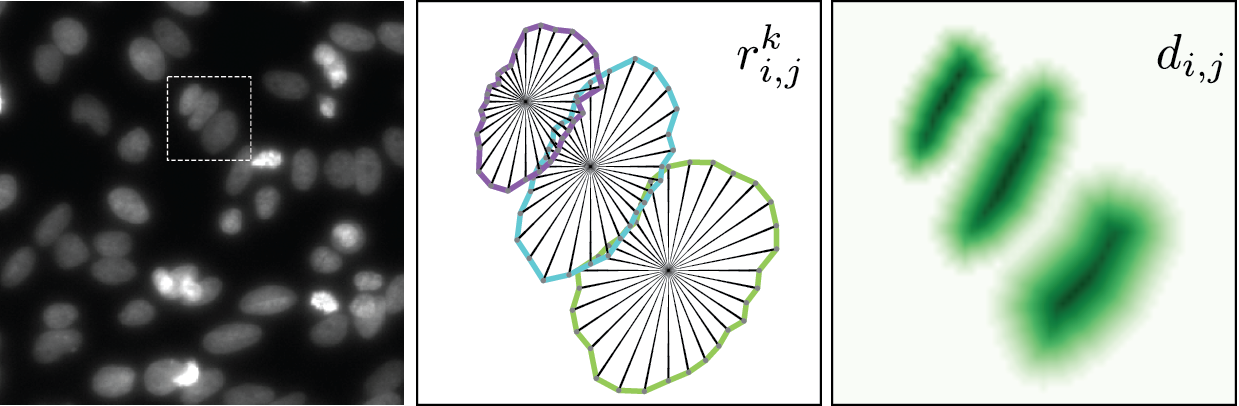
\includegraphics[width=\textwidth]{"images/star_convexity_explained.png"}
	\caption[\texttt{StarDist} summarized]{Example of an area that is complicated to segment due to overlaps. \texttt{StarDist} creates the segementation by forming star-convex polygons and computing the probability to belong to said instance. Source: \Cite{schmidt2018}.}
	\label{figstardistexplained}
\end{figure}

In \stardist, the \texttt{U-Net} architecture \cite{RonnebergerFB15} is used as the backbone and is slightly modified by adding another 128-channel 3x3-convolutional layer with ReLu activation to the \texttt{U-Net} output in order to add a lot of flexibility to the network. This output, in turn, is fed into two other convolutional layers. The first one it is input into is a single channel convolutional layer with sigmoid activation meant to learn object probabilities. The second one has a linear activation and as many channels as there are radial directions. In total, $n+1$ values are predicted for each pixel. Presumably, two points close by will learn two similar representations for the same instance, a way too remove redundant predictions is needed. This is accomplished through non-maximum suppression (NMS) \cite{hosang2017learning, ren2016faster} where only polygons associated with high probability pixels are taken into account.